\section{Tương giao đường thẳng, mặt phẳng, mặt cầu, cực trị}
\subsection{Kiến thức cần nhớ}
\begin{khung}
\subsubsection{Vị trí tương đối của hai mặt phẳng}
	Cho hai mặt phẳng $(P)\colon A_1x+B_1y+C_1z+D_1=0$ và $(Q)\colon A_2x+B_2y+C_2z+D_2=0$.
	\begin{multicols}{2}
		\begin{itemize}
			\item $(P)$ cắt $(Q)\Leftrightarrow \dfrac{A_1}{A_2}=\dfrac{B_1}{B_2}\neq \dfrac{C_1}{C_2}\neq \dfrac{D_1}{D_2}$.
			\item $(P)\parallel(Q)\Leftrightarrow \dfrac{A_1}{A_2}=\dfrac{B_1}{B_2}= \dfrac{C_1}{C_2}\neq \dfrac{D_1}{D_2}$.
			\item $(P)\equiv (Q)\Leftrightarrow \dfrac{A_1}{A_2}=\dfrac{B_1}{B_2}= \dfrac{C_1}{C_2}=\dfrac{D_1}{D_2}$.
			\item $(P)\perp (Q)\Leftrightarrow A_1A_2+B_1B_2+C_1C_2=~0$.
		\end{itemize}
	\end{multicols}
\subsubsection{Vị trí tương đối giữa mặt phẳng và mặt cầu}
	Cho mặt cầu $S(I;R)$ và mặt phẳng $(P)$. Gọi $H$ là hình chiếu vuông góc của $I$ lên $(P)$ và có $d=IH$ là khoảng cách từ $I$ đến mặt phẳng $(P)$. Khi đó : \\
	\begin{tabular}{|m{4cm}|m{5cm}|m{5cm}|}
		\hline
		Nếu $d>R$: Mặt cầu và mặt phẳng không có điểm chung. & Nếu $d=R$: Mặt phẳng tiếp xúc mặt cầu. Lúc đó $(P)$ là mặt phẳng tiếp diện của mặt cầu $(S)$ và $H$ là tiếp điểm. & Nếu $d<R$: Mặt phẳng $(P)$ cắt mặt cầu theo thiết diện là đường tròn có tâm $H$ và bán kính là $r'=~\sqrt{R^2-IH^2}$.\\
		\hline
		% \begin{tikzpicture}[scale=0.6,>=stealth, font=\footnotesize, line join=round, line cap=round]
			% \clip (-3.2,-4) rectangle (3,2.2);
			% \def \x{2} %bán kính trục lớn elip
			% \def \y{0.8} %bán kính trục bé elip
			% \coordinate (I) at (0,0);
			% \coordinate (B) at (\x,0);
			% \coordinate (A) at (-\x,0);
			% \coordinate (M) at (-90:\x);
			% \coordinate (H) at ($(M)-(0,0.6)$);
			% \coordinate (m) at ($(M)+(-\x-1,-\y-0.7)$);
			% \coordinate (n) at ($(M)+(\x-0.2,-\y-0.7)$);
			% \coordinate (p) at ($(M)+(\x+0.7,\y-0.7)$);
			% \coordinate (q) at ($(m)+(p)-(n)$);
			% \tkzDrawCircle[radius](I,A)
			% \draw[dashed] (A)--(B) arc (0:180:\x cm and \y cm);
			% \draw (B) arc (0:-180:\x cm and \y cm);
			% \tkzInterLC(p,q)(I,A)\tkzGetPoints{p'}{q'}
			% \tkzDrawSegments[dashed](p',q' I,M)
			% \tkzDrawSegments(q',q q,m m,n n,p p,p' M,H)
			% \tkzDrawPoints[fill=black](I,H)
			% \tkzLabelPoints[above](I)
			% \tkzLabelPoints[left](H)
			% \pic["$P$",draw,angle radius=6mm,angle eccentricity=0.5]{angle=n--m--q};
			% \node at (-1,0)[above]{$R$};
			% \draw ($(H)+(90:0.2)$)--++(0.2,0)--+(0,-0.2);
			%  \end{tikzpicture}&\begin{tikzpicture}[scale=0.6,>=stealth, font=\footnotesize, line join=round, line cap=round]
			%  \clip (-3.2,-3.3) rectangle (3,2.3);
			%  \def \x{2} %bán kính trục lớn elip
			%  \def \y{0.8} %bán kính trục bé elip
			%  \coordinate (I) at (0,0);
			%  \coordinate (B) at (\x,0);
			%  \coordinate (A) at (-\x,0);
			%  \coordinate (H) at (-90:\x);
			%  \coordinate (m) at ($(H)+(-\x-1,-\y)$);
			%  \coordinate (n) at ($(H)+(\x-0.2,-\y)$);
			%  \coordinate (p) at ($(H)+(\x+0.7,\y)$);
			%  \coordinate (q) at ($(m)+(p)-(n)$);
			%  \tkzDrawCircle[radius](I,A)
			%  \draw[dashed] (A)--(B) arc (0:180:\x cm and \y cm);
			%  \draw (B) arc (0:-180:\x cm and \y cm);
			%  \tkzInterLC(p,q)(I,A)\tkzGetPoints{p'}{q'}
			%  \tkzDrawSegments[dashed](p',q' I,H)
			%  \tkzDrawSegments(q',q q,m m,n n,p p,p')
			%  \tkzDrawPoints[fill=black](I,H)
			%  \tkzLabelPoints[above](I)
			%  \tkzLabelPoints[below](H)
			% \pic["$P$",draw,angle radius=6mm,angle eccentricity=0.5]{angle=n--m--q};
			%  \node at (-1,0)[above]{$R$};
			%  \draw ($(H)+(90:0.2)$)--++(0.2,0)--+(0,-0.2);
			%   \end{tikzpicture}
		% & \begin{tikzpicture}[scale=0.7,>=stealth, font=\footnotesize, line join=round, line cap=round]
			% \clip (-3.2,-3.3) rectangle (3,2.6);
			% \def \x{2} %bán kính trục lớn elip
			% \def \y{0.7} %bán kính trục bé elip
			% \coordinate (I) at (0,0);
			% \coordinate (B) at (\x,0);
			% \coordinate (A) at (-\x,0);
			% \coordinate (H) at ($(0,-0.5*\x)+(0,0.05)$);
			% \coordinate (M) at ($(H)+(-60:\x*0.866 cm and \y*0.866 cm)$);
			% \coordinate (m) at ($(H)+(-\x-1.1,-\y)$);
			% \coordinate (n) at ($(H)+(\x+0.1,-\y)$);
			% \coordinate (p) at ($(H)+(\x+0.9,\y)$);
			% \coordinate (q) at ($(m)+(p)-(n)$);
			% \tkzInterLC(p,q)(I,A)\tkzGetPoints{p'}{q'}
			% \tkzInterLC(m,n)(I,A)\tkzGetPoints{x}{y}
			% \draw (-34:\x) arc (-34:214:\x);
			% \draw (y) arc (-124:-56:\x);
			% \draw (x)[dashed] arc (-56:-30:\x);
			% \draw (y)[dashed] arc (-124:-150:\x);
			% \draw[dashed] ($(-30:\x)+(0,0.05)$) arc (0:180:\x*0.866 cm and \y*0.866 cm);
			% \draw ($(-30:\x)+(0,0.05)$) arc (0:-180:\x*0.866 cm and \y*0.866 cm);
			% \draw[dashed] (p')--(q') (I)--(H) (I)--(M) (H)--(M);
			% \tkzDrawSegments(q',q q,m m,n n,p p,p')
			% \tkzDrawPoints[fill=black](I,H,M)
			% \tkzLabelPoints[above](I)
			% \tkzLabelPoints[left](H)
			% \node at ($(M)+(0.2,0.25)$) {$M$};
			% \pic["$P$",draw,angle radius=6mm,angle eccentricity=0.5]{angle=n--m--q};
			% \path (I)--(M) node[right,midway]{\footnotesize $R$} (H)--(M) node[left,midway]{\footnotesize $r'$};
			% \draw ($(H)+(90:0.2)$)--++(0.2,0)--+(0,-0.2);
			%  \end{tikzpicture}
%		\\
%		\hline
	\end{tabular}
\subsubsection{Vị trí tương đối}
\begin{itemize}
	\item[a.] Vị trí tương đối của hai đường thẳng $d\colon \heva{&x_0+a_1t=0\\&y_0+a_2t=0\\&z_0+a_3t=0}$ và $d'\colon \heva{&x'_0+a'_1t'=0\\&y_0'+a'_2t'=0\\&z'_0+a'_3t'=0.}$
	\begin{itemize}
		\item[\textbf{PP 1}]: Xét hệ phương trình với hai ẩn là $t$ và $t'$ tức xét $\heva{&x_0+a_1t=x'_0+a'_1t'\\&y_0+a_2t=y_0'+a'_2t'\\&z_0+a_3t=z'_0+a'_3t'.}$
		\begin{itemize}
			\item Nếu hệ có nghiệm duy nhất thì $d$ và $d'$ cắt nhau.
			\item Nếu hệ có vô số nghiệm thì $d \equiv d'$.
			\item Nếu hệ vô nghiệm thì $d\parallel d'$ hoặc $d$, $d'$ chéo nhau.
			\begin{itemize}
				\item $\vec{u}_d$ và $\vec{u}_{d'}$ cùng phương thì $d\parallel d'$.
				\item $\vec{u}_d$ và $\vec{u}_{d'}$ không cùng phương thì $d$, $d'$ chéo nhau.
			\end{itemize}
		\end{itemize}
		\item[\textbf{PP 2}]: Xét điểm $M(x_0;y_0;z_0)\in d$, $M'(x'_0;y'_0;z'_0)\in d'$ và $\vec{u}_d$, $\vec{u}_{d'}$.
		\begin{itemize}
			\item $d\parallel d'\Leftrightarrow \heva{&\vec{u}_d=\mathrm{k}\vec{u}_{d'}\\& M \notin d'.}$
			\item $d \equiv d'\Leftrightarrow \heva{&\vec{u}_d=\mathrm{k}\vec{u}_{d'}\\&M\in d'.}$
			\item $d$ cắt $d'\Leftrightarrow \heva{&\vec{u}_d \; \text{không cùng phương với}\; \vec{u}_{d'}\\&\left[ \vec{u}_d, \, \vec{u}_{d'}\right]\cdot \vec{MM'}=0}$.
			\item $d$ chéo $d' \Leftrightarrow \left[\vec{u}_d, \vec{u}_{d'} \right]\cdot \vec{MM'}\ne 0$. 
		\end{itemize}
	\end{itemize}
	\item[b.] \textbf{Vị trí tương đối giữa đường thẳng và mặt phẳng}\\
	Cho đường thẳng $d\colon\heva{&x=x_0+a_1t\\&y=y_0+a_2t\\&z=z_0+a_3t}$ và mặt phẳng $(\alpha)\colon Ax+By+Cz+D=0$.\\
\end{itemize}
\begin{multicols}{2}
	Xét hệ phương trình  $\heva{&x=x_0+a_1t&(1)\\&y=y_0+a_2t&(2)\\&z=z_0+a_3t&(3)\\&Ax+By+Cz+D=0&(4)}\;(*)$
	\columnbreak
	\begin{flushright}
		\begin{tikzpicture}[thick]
			\draw (4,0) coordinate (a)--(0,0)coordinate (b)--(1,2)coordinate (c)--(5,2)coordinate (d)--(4,0)
			pic[draw=black,angle eccentricity=1.2,angle radius=1cm] {angle=a--b--c};
			\draw (.55,.3) node[] {\footnotesize $(\alpha)$};
			\draw[->] (2,1) coordinate (x)--(2,2.7) coordinate (y)node[left]{$\vec{u}_d$};
			\draw (2.2,1)--(2.2,3)node[right]{$d$};
			\draw (1.8,1)--(1.8,1.2)--(2,1.2);
			\draw[->] (3,1) coordinate (x)--(3,2.7) coordinate (y)node[right]{$\vec{n}_\alpha$};
			\draw (3.2,1)--(3.2,1.2)--(3,1.2);
		\end{tikzpicture}
	\end{flushright}
\end{multicols}
\begin{multicols}{2}
	Lấy $(1)$, $(2)$, $(3)$ thế vào $(4)$
	\begin{itemize}
		\item Nếu $(*)$ có nghiệm duy nhất $\Leftrightarrow d$ cắt $(\alpha)$.
		\item Nếu $(*)$ vô nghiệm $\Leftrightarrow d\parallel(\alpha)$.
		\item Nếu $(*)$ vô số nghiệm $\Leftrightarrow d \subset (\alpha)$.
	\end{itemize}
	\columnbreak
	\begin{flushright}
		\begin{tikzpicture}[thick]
			\draw (4,0) coordinate (a)--(0,0)coordinate (b)--(1,2)coordinate (c)--(5,2)coordinate (d)--(4,0)
			pic[draw=black,angle eccentricity=1.2,angle radius=1cm] {angle=a--b--c};
			\draw (.55,.3) node[] {\footnotesize $(\alpha)$};
			\draw[->] (2,1) coordinate (x)--(2,3) coordinate (y)node[left]{$\vec{n}_\alpha$};
			\draw (1.8,1)--(1.8,1.2)--(2,1.2);
			\draw (.5,2.3)--(4.5,2.3)node[above]{$d$};
			\draw[->] (.5,2.6)--(3.8,2.6)node[above]{$\vec{u}_d$};
		\end{tikzpicture}
	\end{flushright}
\end{multicols}
\begin{itemize}
	\item[c.] \textbf{Vị trí tương đối giữa đường thẳng $d$ và mặt cầu $(S)$}
\end{itemize}
Cho mặt cầu $(S)$ có tâm $I$, bán kính $R$ và đường thẳng $\Delta$. Để xét vị trí tương đối giữa $\Delta$ và $(S)$ ta tính $\mathrm{d}(I,\,\Delta)$ rồi so sánh với bán kính $R$.
\immini{
	\begin{itemize}
		\item Nếu $\mathrm{d}(I,\,\Delta)>R$ thì $\Delta$ không cắt $(S)$.
		\item Nếu $\mathrm{d}(I,\,\Delta)=R$ thì $\Delta$ tiếp xúc với $(S)$ tại điểm $H$. 
		\item Nếu $\mathrm{d}(I,\,\Delta)<R$ thì $\Delta$ cắt $(S)$ tại hai điểm $A$, $B$.
	\end{itemize}
}
{
	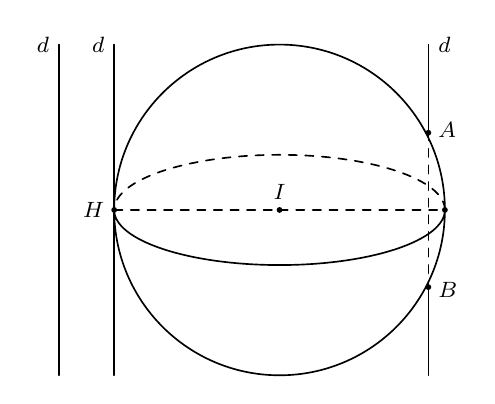
\begin{tikzpicture}[line join=round,line cap=round,line width=.6pt,font=\footnotesize,scale=.7]
		\coordinate[label=above:$I$] (O) at (0,0);
		\coordinate (A) at (3,0);
		\draw (O) circle (3) (A) arc (0:-180: 3 and 1);
		\draw[dashed] (O)--(A) arc (0:180:3 and 1);
		\fill (O)circle(1.5pt) (A)circle(1.5pt);
		\draw[dashed] (-3,0)node[left]{$H$}--(O);
		\draw (-3,-3)--(-3,3)node[left]{$d$};
		\draw (2.7,-3)--(2.7,-1.45) (2.7,1.45)node[right]{$A$}--(2.7,3)node[right]{$d$};
		\draw[dashed](2.7,-1.45)node[right]{$B$}--(2.7,1.45);
		\draw (-4,3)node[left]{$d$}--(-4,-3);
		\fill (-3,0) circle (1.5pt) (2.7,1.4)  circle (1.5pt) (2.7,-1.4)  circle (1.5pt);
	\end{tikzpicture}
}
\end{khung}

\subsection{Bài tập mẫu}
\Opensolutionfile{ans}[ans/ANS-DANG-47]
\begin{khung}
	\begin{vd}%[2H3K3-7][Đề minh họa BGD 2022-2023]
		Trong không gian $Oxyz$, cho mặt cầu $(S)\colon(x-1)^2+y^2+(z-4)^2=9$. Từ điểm $A(4;0;1)$ nằm ngoài mặt cầu, kẻ một tiếp tuyến bất kỳ đến $(S)$ với tiếp điểm $M$. Tập hợp $M$ là đường tròn có bán kính bằng
	\choice
	{ $\dfrac{3}{2}$}
	{\True $\dfrac{3\sqrt{2}}{2}$}
	{ $\dfrac{3\sqrt{3}}{2}$}
	{ $\dfrac{5}{2}$}
	\loigiai{
		\immini{
			Mặt cầu $(S)$ có tâm $I(1;0;4)$ và $R=3$.\\
			Gọi $H$ là hình chiếu vuông góc của $M$ lên đường thẳng $AI$.\\
			Khi đó tập hợp $M$ là đường tròn có bán kính bằng độ dài đoạn $HM$.\\
			Ta có\\
			$AI=3\sqrt{2}$.
			$AM=\sqrt{A{I^2}-MI^2}=3$.
			$MH=\dfrac{MA.MI}{AI}=\dfrac{3\sqrt{2}}{2}$.\\
			Vậy tập hợp $M$ là đường tròn có bán kính bằng $\dfrac{3\sqrt{2}}{2}$.
		}
		{
			\begin{tikzpicture}[line cap=round,line join=round,font=\footnotesize,>=stealth, scale = 1]
				\def \R{2}
				\path 
				(0:0) coordinate (I)
				+(0:\R) coordinate (M)
				(M)++(90:1.5*\R)coordinate(A)
				($(I)!(M)!(A)$)coordinate(H)
				;
				\draw (I) circle (\R)
				(A)--(I)--(M)--cycle
				(M)--(H)
				;
				\foreach \x/\g in {I/-90,M/0,A/90,H/180}
				\fill (\x) circle (1pt)
				+(\g:3mm) node {$\x$};
			\end{tikzpicture}
		}
	}
	\end{vd}
\end{khung}
\subsection{Bài tập tương tự và phát triển}
\begin{ex}%[2H3G3-7]
	Trong không gian tọa độ $Oxyz$, cho hai điểm $A(1;0;0)$, $B(5;6;0)$ và $M$ là điểm thay đổi trên mặt cầu $(S)\colon x^2+y^2+z^2=1$. Tập hợp các điểm $M$ trên mặt cầu $(S)$ thỏa mãn $3MA^2+MB^2=48$ có bao nhiêu phần tử?
\choice
{ $2$}
{ $3$}
{ $0$}
{\True $1$}
\loigiai{
	\textbf{Cách 1.}
	\begin{itemize}
		\item Mặt cầu $(S)\colon x^2+y^2+z^2=1$ có tâm $O\left( 0;0;0 \right)$, bán kính $R=1$.
		\item Ta tìm điểm $I(x;y;z)$ thỏa mãn $3\overrightarrow{IA}+\overrightarrow{IB}=\overrightarrow{0}$.
		\item Có $\overrightarrow{IA}=\left( 1-x;-y;-z \right)$, $\overrightarrow{IB}=\left( 5-x;6-y;-z \right)$.
		\item $3\overrightarrow{IA}+\overrightarrow{IB}=\overrightarrow{0}\Leftrightarrow \left\{ \begin{aligned}
			& 3\left( 1-x \right)+5-x=0 \\
			& 3\left( -y \right)+6-y=0 \\
			& 3\left( -z \right)-z=0 \\
		\end{aligned} \right.\Leftrightarrow \left\{ \begin{aligned}
			& -4x+8=0 \\
			& -4y+6=0 \\
			& -4z=0 \\
		\end{aligned} \right.\Leftrightarrow \left\{ \begin{aligned}
			& x=2 \\
			& y=\dfrac{3}{2} \\
			& z=0 \\
		\end{aligned} \right.\Leftrightarrow I\left( 2;\dfrac{3}{2};0 \right)$.\\
		Suy ra $IA=\dfrac{\sqrt{13}}{2}$, $IB=\dfrac{3\sqrt{13}}{2}$.
		\item Do đó 
		\allowdisplaybreaks
		\begin{eqnarray*}
			3MA^2+MB^2=48&\Leftrightarrow& 3MA^2+MB^2=48\\
			&\Leftrightarrow& 3\left( \overrightarrow{MI}+\overrightarrow{IA} \right)^2+\left( \overrightarrow{MI}+\overrightarrow{IB} \right)^2=48\\
			&\Leftrightarrow& 4MI^2+3IA^2+IB^2+2\overrightarrow{MI}\left( 3\overrightarrow{IA}+\overrightarrow{IB} \right)=48\\
			&\Leftrightarrow& 4MI^2+3IA^2+IB^2=48\\
			&\Leftrightarrow& MI=\dfrac{3}{2}.
		\end{eqnarray*}
	\end{itemize}
	Ta thấy $OI=\dfrac{5}{2}$ nên điểm $I$ nằm ngoài mặt cầu $(S)$.\\
	Ta có $OI=R+MI=OM+MI$, suy ra có một điểm $M$ thuộc đoạn $OI$ thỏa mãn đề bài (điểm $M$ là giao điểm của đoạn thẳng $OI$ và mặt cầu $(S)$).\\
	\textbf{Cách 2.}\\
	Gọi $M(x_0;y_0;z_0)$ thuộc mặt cầu $(S)$ và thỏa mãn $3MA^2+MB^2=48$.\\
	Ta có
	\allowdisplaybreaks
	\begin{eqnarray*}
		3MA^2+MB^2=48&\Leftrightarrow& 3\left[ (x_0-1)^2+y_0^2+z_0^2 \right]+\left[ (x_0-5)^2+(y_0-6)^2+z_0^2 \right]=48\\
		&\Leftrightarrow& 4x_0^2+4y_0^2+4z_0^2-16x_0-12y_0+16=0\\
		&\Leftrightarrow& x_0^2+y_0^2+z_0^2-4x_0-3y_0+4=0.
	\end{eqnarray*}
	Suy ra $M$ thuộc mặt cầu $(S')$ tâm $I'\left( 2;\dfrac{3}{2};0 \right)$, bán kính $R'=\dfrac{3}{2}$.\\
	Mặt khác $M$ thuộc mặt cầu $(S)$ tâm $O\left( 0;0;0 \right)$, bán kính $R=1$.\\
	Ta thấy $OI'=\dfrac{5}{2}=R+R'\Rightarrow $ mặt cầu $(S)$ và $(S')$ tiếp xúc ngoài nhau tại $M$.\\
	Vậy có duy nhất một điểm $M$ thỏa mãn đề bài.
}
\end{ex}

\begin{ex}%[2H3G3-7]
Trong không gian với hệ tọa độ $Oxyz$, cho ba điểm $P$, $Q$, $R$ lần lượt di động trên ba trục tọa độ $Ox$, $Oy$, $Oz$ ( không trùng với gốc tọa độ $O$ ) sao cho $\dfrac{1}{OP^2}+\dfrac{1}{OQ^2}+\dfrac{1}{OR^2}=\dfrac{1}{8}$. Biết mặt phẳng $\left( PQR \right)$ luôn tiếp xúc với mặt cầu $(S)$ cố định. Đường thẳng $d$ thay đổi nhưng luôn đi qua $M\left( \dfrac{1}{2};\dfrac{\sqrt{3}}{2};0 \right)$ và cắt $(S)$ tại hai điểm $A$, $B$ phân biệt. Diện tích lớn nhất của tam giác $AOB$ là
\choice
{ $\sqrt{5}$}
{ $\sqrt{17}$}
{\True $\sqrt{7}$}
{ $\sqrt{15}$}
\loigiai{
	\begin{center}
		\begin{tikzpicture}[>=stealth, line join=round, line cap=round, font=\footnotesize, scale=1]
		\def\r{3}
		\draw[dashed,thick] 
		(180:\r) arc (180:0:{\r} and {0.3*\r});
		%		(90:\r)  arc (90:-90:{0.3*\r} and {\r});
		\draw [thick]	
		(180:\r) arc (180:360:{\r} and {0.3*\r});
		%		(90:\r)  arc (90:360-90:{0.3*\r} and {\r});
		\draw[thick] 
		(0:0) circle(\r);	
		\path
		(0,0) coordinate (O)
		(30:3) coordinate (B)
		(130:3) coordinate (A)
		($(A)!(O)!(B)$) coordinate (I)
		($(A)!0.3!(I)$) coordinate (M)
		(M)--(A)--([turn]0:.5) coordinate (F)
		(I)--(B)--([turn]0:1) coordinate (E)
		;
		\draw[thick] (A)--(F) (B)--(E)node[above]{$ d $};
		\draw[dashed,thick] (A)--(B)--(O)--(A) (M)--(O)--(I) ;
		\foreach \t/\g in {A/130,M/90,I/90,B/80,O/-90}{
			\draw[fill=black] (\t) circle (1pt) node[shift={(\g:7pt)},font=\scriptsize]{$ \t $};
		}
		\draw pic[draw,angle radius=2mm]{right angle=O--I--A};%Theo chiều dương
	\end{tikzpicture}
	\end{center}
	Gọi $H$ là hình chiếu vuông góc của điểm $O$ trên mặt phẳng $\left( PQR \right)$.\\
	Dễ thấy $\dfrac{1}{OH^2}=\dfrac{1}{OP^2}+\dfrac{1}{OQ^2}+\dfrac{1}{OR^2}$ suy ra $\dfrac{1}{OH^2}=\dfrac{1}{8}$ hay $OH=2\sqrt{2}$.\\
	Khi đó suy ra mặt phẳng $\left( PQR \right)$ luôn tiếp xúc với mặt cầu $(S)$ tâm $O$, bán kính $R=2\sqrt{2}$.\\
	Ta có $OM=\sqrt{\dfrac{1}{4}+\dfrac{3}{4}+0}=1<R$ nên điểm $M$ nằm trong mặt cầu $(S)$.\\
	Gọi $I$ là trung điểm của $AB$, do tam giác $OAB$ cân tại $O$ nên ${S_{\triangle OAB}}=\dfrac{1}{2}OI\cdot AB$.\\
	Đặt $OI=x$, vì $OI\le OM$ nên $0<x\le 1$ và $AB=2\sqrt{8-x^2}$.\\
	Ta có ${S_{\triangle OAB}}=\dfrac{1}{2}x\cdot 2\sqrt{8-x^2}=x\sqrt{8-x^2}=\sqrt{8x^2-x^4}$.\\
	Xét hàm số $f(x)=8x^2-x^4$ với $0<x\le 1$.\\
	Có $f'(x)=16x-4x^3=4x\left( 4-x^2 \right)>0$ với mọi $x\in \left( 0;1 \right]\Rightarrow (x)\le f(1)=7$.\\
	Suy ra diện tích của tam giác $OAB$ lớn nhất bằng $\sqrt{7}$ đạt được khi $M$ là trung điểm của $AB$.
}
\end{ex}
\begin{ex}%[2H3G3-7]
	Trong không gian $Oxyz$, cho đường thẳng $\Delta \colon\left\{ \begin{aligned}
	& x=9+3a+at \\
	& y=4+3b+bt \\
	& z=4+6a-6b+2\left( a-b \right)t \\
\end{aligned} \right.\left( t\in \mathbb{R} \right)$. Gọi $(S)$ là mặt cầu tâm $O$, có bán kính nhỏ nhất và tiếp xúc với $\Delta $. Khi đó $(S)$ đi qua điểm nào sau đây?
\choice
{ $M\left( 1;0;0 \right)$}
{ $N\left( \dfrac{1}{2};\dfrac{\sqrt{3}}{2};1 \right)$}
{ $P\left( 0;\dfrac{1}{2};\dfrac{1}{2} \right)$}
{\True $K\left( \dfrac{1}{2};-\dfrac{\sqrt{3}}{2};\sqrt{3} \right)$}
\loigiai{
	Ta có $\left\{ \begin{aligned}
		& x=9+3a+at \\
		& y=4+3b+bt \\
		& z=4+6a-6b+2\left( a-b \right)t \\
	\end{aligned} \right.\left( t\in \mathbb{R} \right)\Leftrightarrow \left\{ \begin{aligned}
		& x=9+a\left( 3+t \right) \\
		& y=4+b\left( 3+t \right) \\
		& z=4+\left( 2a-2b \right).\left( 3+t \right) \\
	\end{aligned} \right.\,\,\,\left( t\in \mathbb{R} \right)$\\
	Đặt $s=3+t\,\,,\,\,s\in \mathbb{R}$. Khi đó $\Delta :\left\{ \begin{aligned}
		& x=9+as \\
		& y=4+bs \\
		& z=4+\left( 2a-2b \right)s \\
	\end{aligned} \right.\left( s\in \mathbb{R} \right)$\\
	Nhận xét $\Delta $ luôn đi qua $A\left( 9;4;4 \right)$ điểm cố định và có véc-tơ chỉ phương $\overrightarrow{u}=\left( a;b;2a-2b \right)$.\\
	Gọi $\overrightarrow{n}=\left( m;n;l \right)\perp \overrightarrow{u}\,\,,\,\,\forall a\,,\,b\left( {m^2}+n^2+l^2>0 \right)$.\\
	Ta có 
	\allowdisplaybreaks
	\begin{eqnarray*}
		ma\,+\,nb\,+2la-2lb=0&\Leftrightarrow& \left( m+2l \right)a+\left( n-2l \right)b=0\\
		&\Leftrightarrow& \left\{ \begin{aligned}
			& m+2l=0 \\
			& n-2l=0 \\
		\end{aligned} \right.\\
		&\Leftrightarrow& \left\{ \begin{aligned}
			& m=-2l \\
			& n=2l \\
		\end{aligned} \right.\\
		&\Rightarrow& \overrightarrow{n}=\left( -2l;2l;l \right)=l\left( 2;-2;-1 \right).
	\end{eqnarray*}
	Do đó $\Delta $ luôn nằm trong mặt phẳng $(P)$ đi qua $A\left( 9;4;4 \right)$ và có một véc-tơ pháp tuyến là $\overrightarrow{n}_P=\left( 2;-2;-1 \right)$.\\
	Phương trình mp $(P)\colon 2x-2y-z-6=0$.\\
	Gọi $K$ là hình chiếu của $O$ trên $\Delta $.\\
	Gọi $H$ là hình chiếu của $O$ trên $(P)$.\\
\immini{
	Ta có $OH\le OK\le OA$.\\
$OK_{\min }=OH=\mathrm{d}\left( O,(P) \right)=\dfrac{|-6|}{\sqrt{2^2+(-2)^2+(-1)^2}}=2$.\\
$OK_{\min }$ khi $K\equiv H\Rightarrow \Delta \equiv AH$.\\
Suy ra, mặt cầu $(S)$ tâm $O$ tiếp xúc $\Delta $ có bán kính nhỏ nhất là $2$.\\
Phương trình mặt cầu tâm $O$ bán kính bằng $2$ là $x^2+y^2+z^2=4$.\\
Vậy $(S)$ luôn đi qua điểm $K\left( \dfrac{1}{2};-\dfrac{\sqrt{3}}{2};\sqrt{3} \right)$.
}
	{	\begin{tikzpicture}[>=stealth, line join=round, line cap=round, font=\footnotesize, scale=.7]
			\path
			(0,0) coordinate (E)
			(0:5) coordinate (F)
			(60:3.3) coordinate (I)
			($(I)+(F)-(E)$) coordinate (G)
			(20:4.5) coordinate (H)
			($(H)+(90:2)$) coordinate (O)
			(15:3) coordinate (K)
			(40:2.2) coordinate (A)
			($(A)!.6!(M)$) coordinate (B)
			(K)--(A)--([turn]0:.5)coordinate (x)
			(A)--(K)--([turn]0:.5)coordinate (y)
			;
			\draw (E)--(F)--(G)--(I)--cycle
			(H)--(O)--(A)--(K)--(H) (K)--(O)
			(x)--(A)--(K)--([turn]0:1)node[above]{$\Delta$}
			;
			\path pic[draw,angle radius=20]{angle=F--E--I}
			(E) node[shift={(25:13pt)}]{$P$};
			%		\draw[dashed] (M)--(H);
			\foreach \t/\g in {O/130,H/-30,K/-130,A/-80}{
				\draw[fill=black] (\t) circle (1pt) node[shift={(\g:7pt)},font=\scriptsize]{$ \t $};
			}
			\draw pic[draw,angle radius=2mm]{right angle=y--K--H};%Theo chiều dương
			\draw pic[draw,angle radius=2mm]{right angle=x--K--O};%Theo chiều dương
			\draw pic[draw,angle radius=2mm]{right angle=O--H--A};%Theo chiều dương
		\end{tikzpicture}
}
}
\end{ex}
\begin{ex}%[2H3G3-7]%
	Trong không gian $Oxyz$, cho mặt phẳng $(P)\colon x+y-z-3=0$ và hai điểm $A(1;1;1)$ và $B(-3;-3;-3)$. Mặt cầu $(S)$ đi qua $A,B$ và tiếp xúc với $(P)$ tại điểm $C$. Biết rằng $C$ luôn thuộc một đường tròn cố định, bán kính đường tròn đó bằng
	\choice
	{$R=4$}
	{$R=\dfrac{2\sqrt{33}}{3}$}
	{\True $R=6$}
	{$\dfrac{2\sqrt{11}}{3}$}
	\loigiai{
		Ta có $\vec{AB} = (-4;-4;-4)=-4(1;1;1)$.\\
		Phương trình đường thẳng $(AB)$ qua $A(1;1;1)$ và có véc-tơ chỉ phương $\vec{u}=(1;1;1)$ dạng $(AB)\colon\heva{&x=1+t\\&y=1+t\\&z=1+t.}$\\
		Gọi $M=AB\cap(P) \Rightarrow M(1+t;1+t;1+t)$. \\
		Vì $M\in (P)$ nên $(1+t)+(1+t)-(1+t)-3=0\Leftrightarrow t= 2$.\\
		Do đó $M(3;3;3) \Rightarrow MA=\sqrt{2^2+2^2+2^2} =2\sqrt{3}$ và $MB=\sqrt{6^2+6^2+6^2} = 6\sqrt{3}$.\\
		Gọi $I$ là tâm mặt cầu $(S)$, theo tính chất của mặt cầu ta có
		\begin{eqnarray*}
			&&MA\cdot MB = MI^2-R_{(S)}^2 \\
			&\Leftrightarrow& 2\sqrt{3}\cdot 6\sqrt{3} = MI^2-IC^2=MC^2\\
			&\Leftrightarrow& MC^2=36 \\
			&\Leftrightarrow& MC = 6.
		\end{eqnarray*}
		Vậy $C$ luôn thuộc đường tròn tâm $M$ bán kính $6$.
	}
\end{ex}
\begin{ex}%[2H3G3-7]
	Trong không gian $Oxyz$, cho mặt cầu $(S)$ có tâm $I\left( -2;1;2 \right)$ và đi qua điểm $A\left( 1;-2;-1 \right)$. Xét các điểm $B$, $C$, $D$ thuộc $(S)$ sao cho $AB$, $AC$, $AD$ đôi một vuông góc với nhau. Thể tích của khối tứ diện $ABCD$ có giá trị lớn nhất bằng
\choice
{\True $36$}
{ $216$}
{ $108$}
{ $72$}
\loigiai{
	Đặt $AB=a$, $AC=b$, $AD=c$ thì $ABCD$ là tứ diện vuông đỉnh $A$, nội tiếp mặt cầu $(S)$.\\
	Khi đó $ABCD$ là tứ diện đặt ở góc $A$ của hình hộp chữ nhật tương ứng có các cạnh $AB$, $AC$, $AD$ và đường chéo $AA'$ là đường kính của cầu.\\
	Ta có $a^2+b^2+c^2=4R^2$.\\
	Xét $V={V_{ABCD}}=\dfrac{1}{6}abc\Leftrightarrow {V^2}=\dfrac{1}{36}{a^2}{b^2}{c^2}$.\\
	Mà $a^2+b^2+c^2\ge 3\sqrt[3]{a^2{b^2}{c^2}}\Leftrightarrow {{\left( \dfrac{a^2+b^2+c^2}{3} \right)}^3}\ge {a^2}{b^2}{c^2}\Leftrightarrow {{\left( \dfrac{4R^2}{3} \right)}^3}\ge 36\cdot V^2\Leftrightarrow V\le {R^3}\cdot\dfrac{4\sqrt{3}}{27}$.\\
	Với $R=IA=3\sqrt{3}$.\\
	Vậy ${V_{\max }}=36$.}
\end{ex}
\begin{ex}%[2H3G3-7]
	Trong không gian với hệ tọa độ $Oxyz$, cho ba điểm $A(0;1;1)$, $B(3;0;-1)$, $C(0;21;-19)$ và mặt cầu $(S)\colon (x-1)^2+(y-1)^2+(z-1)^2=1$. $M(a;b;c)$ là điểm thuộc mặt cầu $(S)$ sao cho biểu thức $ T=3MA^2+2MB^2+MC^2$ đạt giá trị nhỏ nhất. Tính tổng $a+b+c$.
\choice
{\True $a+b+c=\dfrac{14}{5}$}
{ $a+b+c=0$}
{ $a+b+c=\dfrac{12}{5}$}
{ $a+b+c=12$}
\loigiai{
	$(S)\colon (x-1)^2+(y-1)^2+(z-1)^2=1$ có tâm $I\left( 1;1;1 \right)$.\\
	Gọi $G\left( x;y;z \right)$ là điểm thỏa mãn $$3\overrightarrow{GA}+2\overrightarrow{GB}+\overrightarrow{GC}=\overrightarrow{0}\Leftrightarrow \left\{ \begin{aligned}
		& 3\left( 0-x \right)+2\left( 3-x \right)+\left( 0-x \right)=0 \\
		& 3\left( 1-y \right)+2\left( 0-y \right)+\left( 21-y \right)=0 \\
		& 3\left( 1-z \right)+2\left( -1-z \right)+\left( -19-z \right)=0 \\
	\end{aligned} \right.\Leftrightarrow \left\{ \begin{aligned}
		& x=1 \\
		& y=4 \\
		& z=-3 \\
	\end{aligned} \right.\Rightarrow G\left( 1;4;-3 \right).$$
	Ta có
	\allowdisplaybreaks
	\begin{eqnarray*}
		T&=&3MA^2+2MB^2+MC^2\\
		&=&3MG^2+6\overrightarrow{MG}\cdot\overrightarrow{GA}+3GA^2+2MG^2+4\overrightarrow{MG}\cdot\overrightarrow{GB}+2GB^2+MG^2+2\overrightarrow{MG}.\overrightarrow{GC}+GC^2\\
		&=&6MG^2+2\overrightarrow{MG}\left( 3\overrightarrow{GA}+2\overrightarrow{GB}+\overrightarrow{GC} \right)+3GA^2+2GB^2+GC^2\\
		&=&6MG^2+3GA^2+2GB^2+GC^2.
	\end{eqnarray*}
	${T_{\min }}\Leftrightarrow M$ là giao điểm của đường thẳng $IG$ và mặt cầu $(S)$, sao cho $M$ và $G$ cùng phía với $I$.\\
	Phương trình đường thẳng $IG\colon \left\{ \begin{aligned}
		& x=1 \\
		& y=1+3t \\
		& z=1-4t. \\
	\end{aligned} \right.$\\
	$M=IG\cap (S)$ nên tọa độ $M$ là nghiệm của hệ$\left\{ \begin{aligned}
		& x=1 \\
		& y=1+3t \\
		& z=1-4t \\
		& (x-1)^2+(y-1)^2+(z-1)^2=1 \\
	\end{aligned} \right.\Rightarrow \left[ \begin{aligned}
		& t=\dfrac{1}{5} \\
		& t=\dfrac{-1}{5}. \\
	\end{aligned} \right.$ \\
	Khi đó $\left[ \begin{aligned}
		& {M_1}\left( 1;\dfrac{8}{5};\dfrac{1}{5} \right) \\
		& {M_2}\left( 1;\dfrac{2}{5};\dfrac{9}{5} \right). \\
	\end{aligned} \right.$\\
	Vì $M_1G<M_2G$ nên điểm $M\equiv {M_1}\left( 1;\dfrac{8}{5};\dfrac{1}{5} \right)$.\\
	Vậy $a+b+c=\dfrac{14}{5}$.}
\end{ex}
\begin{ex}%[2H3G3-7]
	Trong không gian $Oxyz$ cho $3$ điểm $A\left( 9;0;0 \right)$, $B\left( 0;6;6 \right)$, $C\left( 0;0;-16 \right)$ và điểm $M$ chạy trên mặt phẳng $(Oxy)$. Tìm giá trị lớn nhất của $S=\left| \left| \overrightarrow{MA}+2\overrightarrow{MB} \right|-3MC \right|$.
\choice
{ $45$}
{ $36$}
{ $30$}
{\True $39$}
\loigiai{
	Gọi $I(a;b;c)$ là điểm thỏa mãn: $\overrightarrow{IA}+2\overrightarrow{IB}=\overrightarrow{0}$.\\
	Ta có $\overrightarrow{IA}=\left( 9-a;-b;-c \right)$, $\overrightarrow{IB}=\left( -a;6-b;6-c \right)$.\\
	$\overrightarrow{IA}+2\overrightarrow{IB}=\overrightarrow{0}\Leftrightarrow \overrightarrow{IA}=-2\overrightarrow{IB}\Leftrightarrow \left\{ \begin{matrix}
		9-a=2a \\
		-b=-12+2b \\
		-c=-12+2c \\
	\end{matrix} \right.\Leftrightarrow \left\{ \begin{matrix}
		a=3 \\
		b=4 \\
		c=4 \\
	\end{matrix} \right.$. Suy ra $I\left( 3;4;4 \right)$.\\
	Ta có $\left| \overrightarrow{MA}+2\overrightarrow{MB} \right|=\left| \overrightarrow{MI}+\overrightarrow{IA}+2\left( \overrightarrow{MI}+\overrightarrow{IB} \right) \right|=\left| 3\overrightarrow{MI}+\left( \overrightarrow{IA}+2\overrightarrow{IB} \right) \right|=3MI$.\\
	Suy ra $S=\left| 3MI-3MC \right|=3\left| MI-MC \right|$.\\
	Cao độ của hai điểm $I,\,C$ trái dấu nên hai điểm $I,\,C$ nằm về hai phía so với mặt phẳng $(Oxy)$.\\
	Gọi $I'$ là điểm đối xứng của $I$ qua mặt phẳng $(Oxy)$. Suy ra $I'\left( 3;4;-4 \right)$.\\
	Với mọi điểm $M\in (Oxy)$ ta luôncó $S=3\left| MI-MC \right|=3\left| MI'-MC \right|\le 3I'C$.\\
	Đẳng thức xảy ra khi và chỉ khi $I'$, $C$, $M$ thẳng hàng.\\
	Suy ra $\max S=3I'C=3\sqrt{(0-3)^2+(0-4)^2+(-16+4)^2}=39$.}
\end{ex}
\begin{ex}%[2H3G3-7]
	Trong không gian với hệ tọa độ $Oxyz$ cho ba điểm $A\left( 8;5;-11 \right)$, $B\left( 5;3;-4 \right)$, $C\left( 1;2;-6 \right)$ và mặt cầu $(S)\colon (x-2)^2+(y-4)^2+(z+1)^2=9$. Gọi điểm $M(a;b;c)$ là điểm trên $(S)$ sao cho $\left| \overrightarrow{MA}-\overrightarrow{MB}-\overrightarrow{MC} \right|$ đạt giá trị nhỏ nhất. Hãy tìm $a+b$.
\choice
{ $9$}
{ $6$}
{\True $2$}
{ $4$}
\loigiai{
	\begin{center}
		\begin{tikzpicture}[>=stealth, line join=round, line cap=round, font=\footnotesize, scale=1]
			\def\r{2}
			\draw[dashed,thick] 
			(180:\r) arc (180:0:{\r} and {0.3*\r});
			%		(90:\r)  arc (90:-90:{0.3*\r} and {\r});
			\draw [thick]	
			(180:\r) arc (180:360:{\r} and {0.3*\r});
			%		(90:\r)  arc (90:360-90:{0.3*\r} and {\r});
			\draw[thick] 
			(0:0) circle(\r);	
			\path
			(0,0) coordinate (I)
			(110:\r) coordinate (N1)
			(-70:\r) coordinate (M)
			($(M)!0.6!180:(I)$) coordinate (N)
			($(N)!0.8!190:(M)$) coordinate (B)
			($ (B)+(150:2.5) $) coordinate (A)
			($ (B)+(60:3) $) coordinate (C)
			;
			\draw[fill=black] (N1) circle (1pt) (M) circle (1pt) ;
			\draw[thick] (M)--(N) (B)--(A)--(C)--(B) (N1)node[above]{$ N_1 $} (M)node[above left]{$ M\equiv N_2 $};
			\draw[dashed,thick] (N1)--(M);
			\foreach \t/\g in {I/180,B/-80,N/45,A/180,C/45}{
				\draw[fill=black] (\t) circle (1pt) node[shift={(\g:7pt)},font=\scriptsize]{$ \t $};
			}
			
		\end{tikzpicture}
	\end{center}
	Gọi $N$ là điểm thỏa mãn $\overrightarrow{NA}-\overrightarrow{NB}-\overrightarrow{NC}=\overrightarrow{0}$, suy ra $N\left( -2;0;1 \right)$.\\
	Khi đó 
	\allowdisplaybreaks
	\begin{eqnarray*}
		\left| \overrightarrow{MA}-\overrightarrow{MB}-\overrightarrow{MC} \right|&=&\left| \left( \overrightarrow{MN}+\overrightarrow{NA} \right)-\left( \overrightarrow{MN}+\overrightarrow{NB} \right)-\left( \overrightarrow{MN}+\overrightarrow{NC} \right) \right|\\
		&=&\left| \left( \overrightarrow{NA}-\overrightarrow{NB}-\overrightarrow{NC} \right)-\overrightarrow{MN} \right|\\
		&=&MN.
	\end{eqnarray*}
	Suy ra $\left| \overrightarrow{MA}-\overrightarrow{MB}-\overrightarrow{MC} \right|$ nhỏ nhất khi $MN$ nhỏ nhất.\\
	Mặt cầu $(S)$ có tâm $I\left( 2;4;-1 \right)$, suy ra
	$\overrightarrow{NI}=\left( 4;4;-2 \right)=\left( 2;2;-1 \right)$.\\
	Phương trình $NI=\left\{ \begin{matrix}
		x=2+2t \\
		y=4+2t \\
		z=-1-t. \\
	\end{matrix} \right.$ \\
	hay phương trình $NI$ vào phương trình $(S)$ ta được $${{\left( 2t \right)}^2}+{{\left( 2t \right)}^2}+{{\left( -t \right)}^2}=9\Leftrightarrow {t^2}=1\Leftrightarrow \left[ \begin{matrix}
		t=1 \\
		t=-1. \\
	\end{matrix} \right.$$
	Suy ra $NI$ cắt $(S)$ tại hai điểm phân biệt $N_1\left( 3;6;-2 \right)$, $N_2\left( 0;2;0 \right)$.\\
	Vì $NN_1>NN_2$ nên $MN$ nhỏ nhất khi và chỉ khi $M\equiv N_2$.\\
	Vậy $M\left( 0;2;0 \right)$ là điểm cần tìm.\\
	Suy ra $a+b=2.$\\
}
\end{ex}
\begin{ex}%[2H3G3-7]
	Trong không gian $Oxyz$, cho hai mặt phẳng $(\alpha)\colon x-my+z+6m+3=0$ và $(\beta)\colon mx+y-mz+3m-8=0$(với $m$ là tham số thực); hai mặt phẳng này cắt nhau theo giao tuyến là đường thẳng $\Delta $. Gọi ${\Delta }'$ là hình chiếu của $\Delta $ lên mặt phẳng $(Oxy)$. Biết rằng khi $m$ thay đổi thì đường thẳng ${\Delta }'$ luôn tiếp xúc với một mặt cầu cố định có tâm $I(a;b;c)$ thuộc mặt phẳng $(Oxy)$. Tính giá trị biểu thức $P=10a^2-b^2+3c^2$.
\choice
{ $P=9$}
{\True $P=41$}
{ $P=73$}
{ $P=56$}
\loigiai{
	Mặt phẳng $(\alpha):x-my+z+6m+3=0$ có một véc-tơ pháp tuyến là $\overrightarrow{n}_1=\left( 1;-m;1 \right)$, và mặt phẳng $(\beta)\colon mx+y-mz+3m-8=0$ có một véc-tơ pháp tuyến là $\overrightarrow{n}_2=\left( m;1;-m \right)$.\\
	Ta có $M\left( -3m+\dfrac{4}{m}-3;0;-3m-\dfrac{4}{m} \right)\in \Delta =(\alpha)\cap (\beta)$.\\
	$\Delta $ có một véc-tơ chỉ phương là $\overrightarrow{u}=\left[ \overrightarrow{n}_1;\overrightarrow{n}_2 \right]=\left( {m^2}-1;2m;m^2+1 \right)$.\\
	Gọi $(P)$ là mặt phẳng chứa đường thẳng $\Delta $ và vuông góc với mặt phẳng $(Oxy)$.\\
	Khi đó $(P)$ có một véc-tơ pháp tuyến là $\overrightarrow{n}=\left[ \overrightarrow{u};\overrightarrow{k} \right]=\left( 2m;1-m^2;0 \right)$(với $\overrightarrow{k}=\left( 0;0;1 \right)$).\\
	Phương trình mặt phẳng $(P)$ là $2mx+\left( 1-m^2 \right)y+6m^2+6m-8=0$.\\
	Vì $I(a;b;c)\in (Oxy)$ nên $I\left( a;b;0 \right)$.\\
	Theo giả thiết ta suy ra $(P)$ là tiếp diện của mặt cầu (S)
	\allowdisplaybreaks
	\begin{eqnarray*}
		\mathrm{d}\left( I;(P) \right)=R&\Leftrightarrow& \dfrac{\left| 2ma+\left( 1-m^2 \right)b+6m^2+6m-8 \right|}{\sqrt{4m^2+{{\left( 1-m^2 \right)}^2}}}=R>0\\
		&\Leftrightarrow& \dfrac{\left| 2m\left( a+3 \right)+\left( 6-b \right)m^2+b-8 \right|}{m^2+1}=R>0\\
		&\Leftrightarrow& \left[ \begin{aligned}
			& 2m\left( a+3 \right)+\left( 6-b \right)m^2+b-8=R\left( {m^2}+1 \right) \\
			& 2m\left( a+3 \right)+\left( 6-b \right)m^2+b-8=-R\left( {m^2}+1 \right) \\
		\end{aligned} \right.\\
		&\Leftrightarrow& \left[ \begin{aligned}
			& \left\{ \begin{aligned}
				& 2\left( a+3 \right)=0 \\
				& 6-b=R \\
				& b-8=R \\
				& R>0 \\
			\end{aligned} \right. \\
			& \left\{ \begin{aligned}
				& 2\left( a+3 \right)=0 \\
				& 6-b=-R \\
				& b-8=-R \\
				& R>0 \\
			\end{aligned} \right. \\
		\end{aligned} \right.\\
		&\Leftrightarrow& \left[ \begin{aligned}
			& \left\{ \begin{aligned}
				& a=-3 \\
				& 6-b=b-8 \\
				& R=6-b>0 \\
			\end{aligned} \right. \\
			& \left\{ \begin{aligned}
				& a=-3=0 \\
				& 6-b=b-8 \\
				& -R=6-b<0 \\
			\end{aligned} \right. \\
		\end{aligned} \right.\\
		&\Leftrightarrow&\left\{ \begin{aligned}
			& a=-3 \\
			& b=7. \\
		\end{aligned} \right.
	\end{eqnarray*}
	Vậy $I\left( -3;7;0 \right)$, do đó $P=10a^2-b^2+3c^2=41$.}
\end{ex}
\begin{ex}%[2H3G3-7]
	Trong không gian tọa độ $Oxyz$, cho hai điểm $M\left( -2;-2;1 \right)$, $A\left( 1;2;-3 \right)$ và đường thẳng $d\colon\dfrac{x+1}{2}=\dfrac{y-5}{2}=\dfrac{z}{-1}$. Tìm một véc-tơ chỉ phương $\overrightarrow{u}$ của đường thẳng $\Delta $ đi qua $M$, vuông góc với đường thẳng $d$ đồng thời cách điểm $A$ một khoảng bé nhất.
\choice
{\True $\overrightarrow{u}=\left( 1;0;2 \right)$}
{ $\overrightarrow{u}=\left( 1;7;-1 \right)$}
{ $\overrightarrow{u}=\left( 3;4;-4 \right)$}
{ $\overrightarrow{u}=\left( 2;2;-1 \right)$}
\loigiai{
	Gọi $(P)$ là mặt qua $M$ và vuông góc với đường thẳng $d$.\\
	$\overrightarrow{n}_P=\overrightarrow{u}_d=\left( 2;2;-1 \right)$.\\ 
	Do đó, $(P)\colon 2(x+2)+2(y+2)-1(z-1)=0\Leftrightarrow 2x+2y-z+9=0$.\\
	Gọi $d'$ là đường thẳng qua $A$ và vuông góc với mặt phẳng $(P)$: $\overrightarrow{n}_{d'}=\overrightarrow{n}_P=\left( 2;2;-1 \right)$.\\
	Suy ra $d'\colon \left\{ \begin{aligned}
		& x=1+2t \\
		& y=2+2t \\
		& z=-3-t. \\
	\end{aligned} \right.$\\
	Gọi $B$ là giao điểm của $d'$ và $(P)$, ta có
	$$2(1+2t)+2\left( 2+2t \right)+3+t+9=0\Rightarrow 9t=-18\Leftrightarrow t=-2\Rightarrow B(-3;-2;-1).$$
	Kẻ $AH\perp \Delta \Rightarrow AH\ge AB$ nên khoảng cách từ $A$ đến $\Delta $ nhỏ nhất bằng $AB$.\\
	Vậy đường thẳng $\Delta $ đi qua $2$ điểm $M$; $B$ và có véc-tơ chỉ phương $\overrightarrow{u}=\overrightarrow{MB}=(1;0;2)$.}
\end{ex}
\begin{ex}%[2H3K3-7]
	Trong không gian $Oxyz$, cho biết có hai mặt cầu có tâm nằm trên đường thẳng $d\colon \dfrac{x}{2}=\dfrac{y-1}{1}=\dfrac{z+2}{-1}$, tiếp xúc đồng thời với hai mặt phẳng $(\alpha)\colon x+2y-2z+1=0$ và $(\beta)\colon 2x-3y-6z-2=0$. Gọi $R_1$, $R_2$ $\left(R_1>R_2\right)$  là bán kính của hai mặt cầu đó. Tỉ số $\dfrac{R_1}{R_2}$ bằng
	\choice
	{$\sqrt{2}$}
	{\True $3$}
	{$2$}
	{$\sqrt{3}$}
	\loigiai{
		Gọi $(S)$ là mặt cầu có tâm $I\in d$ tiếp xúc với cả hai mặt phẳng $(\alpha)$, $(\beta)$.\\
		Vì $I\in d\colon \dfrac{x}{2}=\dfrac{y-1}{1}=\dfrac{z+2}{-1}\Rightarrow I(2t;t+1;-2-t)$.\\
		Vì $(S)$ tiếp xúc với cả $(\alpha)$ và $(\beta)$ nên
		\begin{eqnarray*}
			&&R=\mathrm{d}(I;(\alpha))=\mathrm{d}(I;(\beta))\\
			&\Leftrightarrow & R=\dfrac{|2t+2(t+1)-2(-t-2)+1|}{\sqrt{1^2+2^2+(-2)^2}}=\dfrac{|2\cdot 2t-3\cdot (t+1)-6\cdot (-t-2)-2|}{\sqrt{2^2+(-3)^2+(-6)^2}}\\
			&\Leftrightarrow& R=\dfrac{|6t+7|}{3}=|t+1|\\
			&\Leftrightarrow & \hoac{& t=-\dfrac{4}{3} \\ & t=-\dfrac{10}{9}.}
		\end{eqnarray*}
		Với $t=-\dfrac{10}{9}\Rightarrow R=\dfrac{1}{9}$, với $t=-\dfrac{4}{3}\Rightarrow R=\dfrac{1}{3}$. Do đó $R_1=\dfrac{1}{3}$, $R_2=\dfrac{1}{9}\Rightarrow \dfrac{R_1}{R_2}=3$.
	}
\end{ex}
\begin{ex}%[2H3G3-7]
Trong không gian với hệ tọa độ $Oxyz$cho điểm $A\left( -2;2;-2 \right)$ và điểm $B\left( 3;-3;3 \right)$. Điểm $M$ thay đổi trong không gian thỏa mãn $\dfrac{MA}{MB}=\dfrac{2}{3}$. Điểm $N(a;b;c)$ thuộc mặt phẳng $(P)\colon -x+2y-2z+6=0$ sao cho $MN$ nhỏ nhất. Tính tổng $ t=a+b+c$.
\choice
{ $6$}
{\True $-2$}
{ $12$}
{ $-6$}
\loigiai{
	Gọi $M(x;y;z)$.\\
	Ta có $\dfrac{MA}{MB}=\dfrac{2}{3}\Leftrightarrow 9MA^2=4MB^2\Leftrightarrow (x+6)^2+(y-6)^2+(z+6)^2=108$.\\
	Vậy điểm $M$ thuộc mặt cầu tâm $I\left( -6;6;-6 \right)$ bán kính $R=6\sqrt{3}$.\\
	Vậy $MN$ nhỏ nhất khi $M$, $N$ thuộc đường thẳng đi qua tâm $I$ và vuông góc với mặt phẳng $(P)$.\\
	Gọi $(d)$ là đường thẳng đi qua tâm $I$ và vuông góc với mặt phẳng $(P)$.\\
	Khi đó $(d)\colon\left\{ \begin{aligned}
		& x=-6-t \\
		& y=6+2t \\
		& z=-6-2t. \\
	\end{aligned} \right.$\\
	Tọa độ điểm $N$ là nghiệm của hệ phương trình
	$$\left\{ \begin{aligned}
		& x=-6-t \\
		& y=6+2t \\
		& z=-6-2t \\
		& -x+2y-2z+6=0 \\
	\end{aligned} \right.\Leftrightarrow \left\{ \begin{aligned}
		& x=-6-t \\
		& y=6+2t \\
		& z=-6-2t \\
		& 6+t+12+4t+12+4t+6=0 \\
	\end{aligned} \right.\Leftrightarrow \left\{ \begin{aligned}
		& x=-2 \\
		& y=-2 \\
		& z=2 \\
		& t=-4. \\
	\end{aligned} \right.$$
	$\Rightarrow N\left( -2;-2;2 \right)$.\\
	Do đó $ t=-2-2+2=-2$.}
\end{ex}
\begin{ex}%[2H3G3-7]
	Trong không gian $Oxyz$, cho mặt phẳng $5$ và ba điểm $A\left( 1;2;1 \right)$, $B\left( 0;1;2 \right)$, $C\left( 0;0;3 \right)$. Điểm $M(x_0;y_0;z_0)$ thuộc $(P)$ sao cho $MA^2+3MB^2+2MC^2$ đạt giá trị nhỏ nhất. Giá trị $x_0+2y_0-z_0$ bằng
\choice
{ $\dfrac{46}{9}$}
{ $\dfrac{4}{9}$}
{\True $\dfrac{2}{9}$}
{ $\dfrac{6}{9}$}
\loigiai{
	Gọi $I$ là điểm thỏa mãn $\overrightarrow{IA}+3\overrightarrow{IB}+2\overrightarrow{IC}=\overrightarrow{0}$ $\Leftrightarrow \overrightarrow{OI}=\dfrac{1}{6}\left( \overrightarrow{OA}+3\overrightarrow{OB}+2\overrightarrow{OC} \right)\Rightarrow I\left( \dfrac{1}{6};\dfrac{5}{6};\dfrac{13}{6} \right)$.\\
	Khi đó, ta có
	\allowdisplaybreaks
	\begin{eqnarray*}
		Q&=&MA^2+3MB^2+2MC^2\\
		&=&{{\left( \overrightarrow{MI}+\overrightarrow{IA} \right)}^2}+3{{\left( \overrightarrow{MI}+\overrightarrow{IB} \right)}^2}+2{{\left( \overrightarrow{MI}+\overrightarrow{IC} \right)}^2}\\
		&=&6MI^2+IA^2+3IB^2+2IC^2.
	\end{eqnarray*}
	Do $IA^2+3IB^2+2IC^2$ không đổi nên $Q$ nhỏ nhất khi $MI$ nhỏ nhất.\\
	Mà $M$ thuộc mặt phẳng $(P)$ nên $MI$ nhỏ nhất khi $M$ là hình chiếu vuông góc của $I$ trên $(P)$.\\
	$MI\perp (P)$ nên phương trình $MI$ là $\left\{ \begin{aligned}
		& x=\dfrac{1}{6}+t \\
		& y=\dfrac{5}{6}+t \\
		& z=\dfrac{13}{6}+t \\
	\end{aligned} \right.$ $\Rightarrow M\left( \dfrac{1}{6}+t;\dfrac{5}{6}+t;\dfrac{13}{6}+t \right)$.\\
	$M\in (P)$ $\Leftrightarrow \dfrac{1}{6}+t+\dfrac{5}{6}+t+\dfrac{13}{6}-4=0\Leftrightarrow t=\dfrac{5}{18}$ $\Rightarrow M\left( \dfrac{4}{9};\dfrac{10}{9};\dfrac{22}{9} \right)$.\\
	Suy ra $x_0+2y_0-z_0=\dfrac{4}{9}+\dfrac{20}{9}-\dfrac{22}{9}=\dfrac{2}{9}$.
}
\end{ex}
\begin{ex}%[2H3G3-7]
Trong không gian với hệ tọa độ $Oxyz$, xét đường thẳng $\Delta $ đi qua điểm $A\left( 0;0;1 \right)$ và vuông góc với mặt phẳng $(Ozx)$. Tính khoảng cách nhỏ nhất giữa điểm $B\left( 0;4;0 \right)$ tới điểm $C$ trong đó $C$ là điểm cách đều đường thẳng $\Delta $ và trục $Ox$.
\choice
{\True $\dfrac{1}{2}$}
{ $3\sqrt{2}$}
{ $\sqrt{6}$}
{ $\dfrac{\sqrt{65}}{2}$}
\loigiai{
	Vì đường thẳng $\Delta $ đi qua điểm $A\left( 0;0;1 \right)$ và vuông góc với mặt phẳng $(Ozx)$ thì $\Delta $ song song với trục $Oy$ và nằm trong mặt phẳng $(Oyz)$.\\
	Dễ thấy $OA$ là đường vuông góc chung của $\Delta $ và $Ox$.\\
	Xét mặt phẳng $(\alpha)$ đi qua $I\left( 0;0;\dfrac{1}{2} \right)$ và là mặt phẳng trung trực của $OA$.\\
	Khi đó $\Delta \parallel (\alpha)$, $Ox \parallel (\alpha)$ và mọi điểm nằm trên $(\alpha)$ có khoảng cách đến $\Delta $ và $Ox$ là bằng nhau.\\
	Vậy tập hợp điểm $C$ là các điểm cách đều đường thẳng $\Delta $ và trục $Ox$ là mặt phẳng $(\alpha)$.\\
	Mặt phẳng $(\alpha)$ đi qua $I\left( 0;0;\dfrac{1}{2} \right)$ có véc-tơ pháp tuyến là $\overrightarrow{k}=\left( 0;0;1 \right)$ nên có phương trình: $z-\dfrac{1}{2}=0$.\\
	Đoạn $BC$ nhỏ nhất khi $C$ là hình chiếu vuông góc của $B$ lên $(\alpha)$.\\
	Do đó khoảng cách nhỏ nhất giữa điểm $B\left( 0;4;0 \right)$ tới điểm $C$ chính là khoảng cách từ $B\left( 0;4;0 \right)$ đến mặt phẳng $(\alpha)$: $z-\dfrac{1}{2}=0$ suy ra $\min \left( BC \right)=d\left( B;(\alpha) \right)=\dfrac{\left| 0-\dfrac{1}{2} \right|}{1}=\dfrac{1}{2}$.}
\end{ex}
\begin{ex}%[2H3G3-7]
	Trong không gian $Oxyz$, cho điểm $M(3;0;4)$ và mặt cầu $(S)\colon (x-1)^2+(y+2)^2+(z-4)^2=9$. Qua điểm $M$ vẽ $3$ tia $Mu$, $Mv$, $Mw$ đôi một vuông góc với nhau và cắt mặt cầu $(S)$ lần lượt tại các điểm $A$, $B$, $C$. Gọi $E$ là đỉnh đối diện với đỉnh $M$ của hình hộp chữ nhật có $3$ cạnh là $MA$, $MB$, $MC$. Biết điểm $E$ luôn thuộc một mặt cầu cố định khi $3$ tia $Mu$, $Mv$, $Mw$ thay đổi thỏa mãn đề bài, tính bán kính mặt cầu đó.
	\choice
	{$\sqrt{13}$}
	{$4\sqrt{2}$}
	{\True $\sqrt{11}$}
	{$2\sqrt{3}$}
	\loigiai{
		\immini
		{
			Theo giả thiết $A,B,C\in (S)$, $E$ là đỉnh đối diện với đỉnh $M$ của hình hộp chữ nhật có $3$ cạnh là $MA$, $MB$, $MC$.\\
			Gọi $I$ là tâm của mặt cầu $(S)$, ta có
			$$\heva{&
				\overrightarrow{ME}=\overrightarrow{MA}+\overrightarrow{MB}+\overrightarrow{MC}\\&
				IA=IB=IC=R=3\\&
				IM=2\sqrt{2}.}$$
			Khi đó:
			\begin{eqnarray*}
				IE^2&=&\left(\overrightarrow{IE}\right)^2=\left(\overrightarrow{IM}+\overrightarrow{ME}\right)^2\\
				&=&\left(\overrightarrow{IM}+\overrightarrow{MA}+\overrightarrow{MB}+\overrightarrow{MC}\right)^2\\
				&=&IM^2+MA^2+MB^2+MC^2+2\overrightarrow{IM}\cdot\left(\overrightarrow{MA}+\overrightarrow{MB}+\overrightarrow{MC}\right)\\
				&=&IM^2+\left(\overrightarrow{MI}+\overrightarrow{IA}\right)^2+\left(\overrightarrow{MI}+\overrightarrow{IB}\right)^2+\left(\overrightarrow{MI}+\overrightarrow{IC}\right)^2+2\overrightarrow{IM}\cdot \left(3\overrightarrow{MI}+\overrightarrow{IA}+\overrightarrow{IB}+\overrightarrow{IC}\right)\\
				&=&IA^2+IB^2+IC^2-2IM^2=11.
			\end{eqnarray*}
			Vậy điểm $E$ luôn thuộc mặt cầu tâm $I$ bán kính $\sqrt{11}$ .
		}
		{
			\begin{tikzpicture}[scale=.7, font=\footnotesize,line join=round, line cap=round,>=stealth]
				\pgfmathsetmacro{\a}{3.8}
				\path (0,0)coordinate (M) (M)++(0,\a) coordinate (A) (M)++(\a,0) coordinate (B) (M)++(-2,-1.5) coordinate (C) (1.2,1) coordinate (I);
				\coordinate (E') at ($(B)+(C)-(M)$);
				\coordinate (E) at ($(E')+(0,\a)$);
				\coordinate (B') at ($(B)+(0,\a)$);
				\coordinate (C') at ($(C)+(0,\a)$);
				\draw[ball color=gray,opacity=0.5] (I) circle (4.2cm);
				\draw[dashed] (M)--(A) (M)--(B) (M)--(C) (M)--(E)--(E') (B)--(E')--(C)--(C')--(E)--(B')--(A)--(C') (B)--(B');
%				\tkzMarkRightAngles(B,M,A A,M,C C,M,B)
				\foreach \d/\g in {M/180,A/90,B/0,C/-120,E/90,I/-90} \draw[fill=black] (\d) circle (1pt) +(\g:0.5) node{$\d$};
			\end{tikzpicture}
		}
	}
\end{ex}
\begin{ex}%[2H3K3-7]
	Trong không gian $Oxyz$, cho bốn điểm $A(2;0;0),B(0;4;0),C(2;4;0),D(0;0;6)$ và mặt cầu $(S)\colon x^2+y^2+z^2-2x-4y-6z=0$. Có bao nhiêu mặt phẳng cắt $(S)$ theo một đường tròn có diện tích $14\pi$ và cách đều năm điểm $O,A,B,C,D$ ($O$ là gốc tọa độ)?
	\choice
	{$5$}
	{\True  $3$}
	{$1$}
	{Vô số}
	\loigiai
	{
		Mặt cầu $(S)$ có tâm $I(1;2;3)$ bán kính $R=\sqrt{14}$.\\
		Gọi $(P)$ là mặt phẳng thỏa yêu cầu bài toán.\\
		Vì $(P)$ cách đều nằm điểm $A,B,C,D,O$ nên $(P)$ không đi qua $O$.\\
		Giả sử $(P)\colon ax+by+cz+2=0$, (với $a^2+b^2+c^2>0$) là mặt phẳng cần tìm.\\
		Gọi $r$ là bán kính của đường tròn trong giao tuyến của $(S)$ và $(P)$.\\
		Vì đường tròn giao tuyến có diện tích là $14\pi $ nên $r=\sqrt{14}=R$.\\
		Do đó tâm $I(1;2;3)$ của mặt cầu $(S)$ nằm trong mặt phẳng $(P)$. Khi đó ta có $a+2b+3c+2=0$.\\
		Do $(P)$ cách đều năm điểm $O,A,B,C,D$ nên
		\begin{eqnarray*}
			&&\dfrac{|2a+2|}{\sqrt{a^2+b^2+c^2}}=\dfrac{|4b+2|}{\sqrt{a^2+b^2+c^2}}=\dfrac{|2a+4b+2|}{\sqrt{a^2+b^2+c^2}}=\dfrac{|6c+2|}{\sqrt{a^2+b^2+c^2}}=\dfrac{2}{\sqrt{a^2+b^2+c^2}}\\
			&\Leftrightarrow &|a+1|=|2b+1|=|a+2b+1|=|3c+1|=1.
		\end{eqnarray*}
		Kết hợp với $a+2b+3c+2=0$ ta có hệ phương trình
		$$\heva{& |a+1|=1\\&|2b+1|=1\\&|3c+1|=1\\&a+2b+3c+2=0 }\Leftrightarrow\hoac{& a=-2,b=c=0\\&a=c=0,b=-1\\&a=b=0,c=-\dfrac{2}{3}. }$$
		Vậy có $3$ mặt phẳng thỏa yêu cầu bài toán.
		
	}
\end{ex}
\begin{ex}%[TT  L1- Ngô Gia Tự, Dak-lak - 22]%[Huỳnh Xuân Tín - 12EX5]%[2H3K3-7]%
	Trong không gian $O x y z$, cho hai mặt phẳng $(P)\colon x-y+2 z+1=0$, $(Q)\colon 2 x+y+z-1=0$. Gọi $(S)$ là mặt cầu có tâm thuộc trục hoành, đồng thời $(S)$ cắt mặt phẳng $(P)$ theo giao tuyến là một đường tròn có bán kính bằng $2$ và $(S)$ cắt mặt phẳng $(Q)$ theo giao tuyến là một đường tròn có bán kính bằng $r$. Xác định $r$ sao cho chỉ đúng một mặt cầu $(S)$ thỏa yêu cầu.
	\choice
	{$r=\dfrac{\sqrt{6}}{2}$}
	{$r=\dfrac{\sqrt{2}}{2}$}
	{\True $r=\dfrac{3 \sqrt{2}}{2}$}
	{$r=\sqrt{3}$}
	\loigiai{
		\immini{Gọi $(S)$ là mặt cầu có tâm $I(a;0;0)\in Ox$ có tâm $R$. Mặt cầu $(S)$ cắt mặt phẳng $(P)$, $(Q)$ là các đường tròn có tâm $A$, $B$.\\
			Ta có
			$\mathrm{d}(I,(P))=IA=\dfrac{|a+1|}{\sqrt{6}}=\sqrt{R^2-4}\Rightarrow \dfrac{(a+1)^2}{6}=R^2-4$.\\
			$\mathrm{d}(I,(Q))=IB=\dfrac{|2a-1|}{\sqrt{6}}=\sqrt{R^2-r^2}\Rightarrow \dfrac{(2a-1)^2}{6}=R^2-r^2$.\\
			Suy ra $r^2-4=\dfrac{(a+1)^2}{6}-\dfrac{(2a-1)^2}{6}\Rightarrow a^2-2a-8+2r^2=0$ (*)\\
			Yêu cầu bài toán thỏa mãn khi (*) có đúng một nghiệm $a$. \\
			Khi đó $\Delta'=0\Leftrightarrow 1+8-2r^2=0\Rightarrow r=\dfrac{3 \sqrt{2}}{2}$.
		}{
			\begin{tikzpicture}[line cap=round,line join=round, font=\footnotesize, >=stealth, scale=1]
				\def\g{70}\def\r{3}
				\path
				(0,0) coordinate (I)
				(0,-\r/2) coordinate  (A)
				(\g-90:\r/2) coordinate (B)
				%	(0,-\r-2) coordinate (A)
				(-2.6,-\r/2) coordinate (K)
				(2.6,-\r/2) coordinate (L)
				%	(intersection of O--L and I--O') coordinate (M)
				;
				\draw (I) circle (\r);
				\draw[dashed,name path=o] (2.6,-\r/2)  arc (0:180:2.6cm and 0.6cm);
				\draw[name path=m] (2.6,-\r/2)  arc (360:180:2.6cm and 0.6cm);
				\draw[name path=l,rotate=\g] (2.6,-\r/2)  arc (360:180:2.6cm and 0.6cm);
				\draw[name path=n,rotate=\g,dashed] (2.6,-\r/2)  arc (0:180:2.6cm and 0.6cm);
				%	\path [red,name intersections={of=l and m,by={E}}];
				%	\path [red,name intersections={of=n and o,by={F}}];
				\draw[dashed] (2.6,-\r/2)--(K)--(I)--(B) (I)--(A);
				%\draw (K)--(A)--(0,-\r) (2.6,-\r/2)--(M)--(\g-90:\r);
				\foreach \d/\g in {I/120,A/135,B/70,K/180}{
					\draw[fill=black](\d) circle (1pt) +(\g:.35)node{$\d$};}
				%\tkzDrawLines[dashed, add=0 and 1.6](O,I O',I)
		\end{tikzpicture}}
	}
\end{ex}
\begin{ex}%[Liên trường THPT Nghệ An 2022]%[Thai Dat, 12EX5]%[2H3K3-7]%
	Trong không gian $Oxyz$, cho mặt cầu $(S)\colon x^2 + y^2 + (z+2)^2 = 16$, điểm $A$ nằm trên đường thẳng $\Delta$ có phương trình $\heva{&x=1+t\\ &y=1+t\\ &z=2}$ và nằm ngoài mặt cầu $(S)$. Từ $A$ kẻ các tiếp tuyến đến mặt cầu $(S)$. Gọi $(P_m)$ là mặt phẳng chứa các tiếp điểm, biết mặt phẳng $(P_m)$ luôn chứa một đường thẳng $d$ cố định. Phương trình đường thẳng $d$ là
	\choice
	{$\heva{&x=t\\ &y=-t\\ &z=-2}$}
	{$\heva{&x=t\\ &y=t\\ &z=2}$}
	{\True $\heva{&x=t\\ &y=-t\\ &z=2}$}
	{$\heva{&x=1+t\\ &y=1-t\\ &z=2}$}
	\loigiai{
		\immini
		{
			Mặt cầu $(S)$ có tâm $I(0;0;-2)$ và bán kính $R=4$.\\
			Gọi $H$ là hình chiếu của $I$ lên đường thẳng $\Delta$. Ta có $H(1+t;1+t;2)$ với $t\in\mathbb{R}$.\\
			Do $IH\perp \Delta$ nên $\vec{IH}\cdot \vec{u}_{\Delta} = 0 \Leftrightarrow t+1 + t+1 = 0 \Leftrightarrow t = -1$. \\
			Suy ra $H(0;0;2)$ và $IH = 4$ nên đường thẳng $\Delta$ tiếp xúc với mặt cầu $(S)$ tại $H$ hay $H\in (P_m)$.\\
			Chọn $d$ là đường thẳng đi qua $H$, vuông góc với mặt phẳng chứa đường thẳng $\Delta$ và điểm $I$. Hiển nhiên $d$ cố định.
		}
		{
			\begin{tikzpicture}[line join=round, line cap = round, >=stealth, scale=.8,font=\footnotesize]
				\path
				(0,0) coordinate (I)
				(0,-2) coordinate (H)
				(-4,-2) coordinate (A)
				($(A)!(H)!(I)$) coordinate (h)
				($(H)!2!(h)$) coordinate (B)
				;
				\draw (I) circle(2) (A)--(I)--(B)--(A) (I)--(H)--(B) (-5,-2)--(2,-2) node[above right]{$\Delta$};
				\foreach \x/\g in {I/45,H/-90,A/-90,B/90}
				\fill[black] (\x) circle(1pt) ($(\x)+(\g:3mm)$) node{$\x$};
			\end{tikzpicture}
		}
		\noindent Khi đó $d \perp IA$, mà $\vec{IA}$ là véc-tơ pháp tuyến của mặt phẳng $(P_m)$ nên $d\parallel (P_m)$ hoặc $d\subset (P_m)$.\\
		Kết hợp với $H\in d$ và $H\in (P_m)$ nên $d\subset (P_m)$.\\
		Ta có $\vec{u}_d = \left[ \vec{u}_\Delta ; \vec{IH}  \right] = (4;-4;0) = 4(1;-1;0)$ nên phương trình tham số của đường thẳng $d$ là
		\[
		\heva{& x=t \\ & y=-t\\ & z=2.}
		\]
	}
\end{ex}
\begin{ex}%[2H3K3-7]%
	Trong không gian $Oxyz$, cho đường thẳng $\Delta\colon \dfrac{x-1}{2}=\dfrac{y}{1}=\dfrac{z-2}{2}$ và điểm $M(2;5;3)$. Mặt phẳng $(P)$ chứa $\Delta$ sao cho khoảng cách từ $M$ đến $(P)$ lớn nhất có phương trình là
	\choice
	{\True $x-4y+z-3=0$}
	{$x+4y-z+1=0$}
	{$x-4y-z+1=0$}
	{$x+4y+z-3=0$}
	\loigiai{
		\immini{
			Gọi $H$ là hình chiếu vuông góc của $M$ lên $(P)$, $I$ là hình chiếu vuông góc của $M$ lên $\Delta$. \\
			Ta có $\triangle MHI$ vuông tại $H$ nên $MH\le MI$, do đó $MH$ đạt giá trị lớn nhất khi $H\equiv I$, khi đó mặt phẳng $(P)$ chứa $\Delta$ và vuông góc với $MI$.
		}
		{
			\begin{tikzpicture}[line join = round, line cap = round,>=stealth,font=\footnotesize,scale=1]
				\path
				(-1,0) coordinate (A)
				(4,0) coordinate (D)
				(0,2.5) coordinate (B)
				($(B)+(D)-(A)$) coordinate (C)
				(1,3.5) coordinate (M)
				(1,1) coordinate (P)
				(4,2) coordinate (Q)
				(2.5,1.5) coordinate (I)
				(1,1.5) coordinate (H)
				;
				\draw (A)--(D)--(C)--(B)--(A) (M)--(H)--(I)--(M);
				\node at (A)[above right]{$P$};
%				\tkzMarkAngles[size=0.7,arc=l](D,A,B)
				\draw (P)--(Q)node[below]{$\Delta$};
%				\tkzMarkRightAngles[size=0.17](M,I,Q)
%				\tkzMarkRightAngles[size=0.17](M,H,I)
				\foreach \x/\g in{M/90,H/-135,I/-90}
				\draw[fill=black](\x)circle(1pt)node[shift={(\g:0.35)}]{$\x$};
			\end{tikzpicture}
		}
		\noindent Ta có $I\in\Delta\Rightarrow I(1+2t;t;2+2t)$, suy ra $\overrightarrow{MI}=(-1+2t;t-5;-1+2t)$. \\
		Có $MI\perp\Delta\Leftrightarrow\overrightarrow{MI}\perp \overrightarrow{u}_{\Delta}=0\Leftrightarrow 2(2t-1)+t-5+2(2t-1)=0\Leftrightarrow t=1$. \\
		Vậy $I(3;1;4)$. \\
		Mặt phẳng $(P)$ đi qua $I$ và có véc-tơ pháp tuyến là $\overrightarrow{MI}=(1;-4;1)$ có phương trình là $$x-3-4(y-1)+z-4=0\Leftrightarrow x-4y+z-3=0.$$
	}
\end{ex}
\begin{ex}%[2H3K3-7]
	Trong không gian $Oxyz$, cho mặt cầu $x^2+y^2+z^2 -2x-2y-2z=0$ và $A(2;2;0)$. Viết phương trình mặt phẳng $(OAB)$ biết $B$ thuộc mặt cầu $(S)$, có hoành độ dương và tam giác $OAB$ đều.
	\choice
	{\True $x-y-z=0$}
	{$x-y-2z=0$}
	{$x-y+z=0$}
	{$x-y+2z=0$}
	\loigiai{
		Giả sử $B(a;b;c)$. Do $B \in (S)$ nên $a^2 + b^2 +c^2 -2a -2b -2c =0$.\\
		Tam giác $OAB$ đều nên 	$\heva{&OA=OB\\&OB=AB} \Leftrightarrow \heva{&a^2+b^2+c^2 = 8\\& a^2+b^2+c^2 =(a-2)^2 +(b-2)^2 +c^2. }$\\
		Do đó ta có hệ $\heva{&a^2 + b^2 +c^2 -2a -2b -2c =0\\ &a^2+b^2+c^2 = 8\\& a^2+b^2+c^2 =(a-2)^2 +(b-2)^2 +c^2 } \Leftrightarrow  \heva{& a+b+c =4 \\ & a+b=2 \\& a^2 + b^2 +c^2 = 8}$\\
		$\Leftrightarrow (a;b;c)= (2;0;2)$ hoặc $(a;b;c)= (0;2;2)$.\\
		Theo giả thiết ta nhận $(a;b;c)= (2;0;2)$. Ta có $\left[ \overrightarrow{OA}, \overrightarrow{OB}\right] = (4;-4;-4)$.\\
		Mặt phẳng $(OAB)$ đi qua điểm $O$ và có véc-tơ pháp tuyến $\overrightarrow{n}= \dfrac{1}{4} \left[ \overrightarrow{OA}, \overrightarrow{OB}\right] = (1;-1;-1)$ nên có phương trình $x-y-z=0$.
		
	}
\end{ex}
\begin{ex}%[2H3K3-7]%
	Trong không gian $Oxyz$, viết phương trình mặt phẳng tiếp xúc với mặt cầu $(S)\colon{(x-1)^2}+y^2+(z+2)^2=6, $ đồng thời song song với hai đường thẳng $d_1\colon\dfrac{x-2}{3}=\dfrac{y-1}{-1}=\dfrac{z-1}{-1}$ và $d_2\colon\dfrac{x}{1}=\dfrac{y+2}{1}=\dfrac{z-2}{-1}$.
	\choice
	{$\hoac{
			& x-y+2z+9=0\\
			& x-y+2z-3=0}$}
	{$x+y+2z+9=0$}
	{\True $\hoac{
			& x+y+2z+9=0\\
			& x+y+2z-3=0}$}
	{$x-y+2z-3=0$}
	\loigiai{
		Mặt cầu $(S)\colon{(x-1)^2}+y^2+(z+2)^2=6$ có tâm $I(1;0;-2)$ và bán kính $r=\sqrt{6}$.\\
		Đường thẳng $d_1$ qua điểm $A(2;1;1)$, nhận véc-tơ  $\overrightarrow{a}=(3;-1;-1)$ làm véc-tơ chỉ phương.\\
		Đường thẳng $d_2$ qua điểm $B(0;-2;2)$, nhận véc-tơ $\overrightarrow{b}=(1;1;-1)$ làm véc-tơ chỉ phương.\\
		Mặt phẳng $(P)$ song song với hai đường thẳng $d_1$ và $d_2$ nên $(P)$ nhận véc-tơ $\overrightarrow{n}=\left[\overrightarrow{a},\overrightarrow{b}\right]=(2;2;4)$ làm véc-tơ pháp tuyến.\\
		Suy ra $(P)$ có phương trình tổng quát dạng $x+y+2z+m=0$.\\
		$(P)$ tiếp xúc với mặt cầu$(S) \Leftrightarrow \mathrm{d}(I,(P))=r\Leftrightarrow\dfrac{\left| 1+0-4+m\right|}{\sqrt{1+1+4}}=\sqrt{6}\Leftrightarrow\left| m-3\right|=6\Leftrightarrow\hoac{
			& m-3=6\\
			& m-3=-6\\
		}\Leftrightarrow\hoac{
			& m=9\\
			& m=-3.}$\\
		Với $m=9$ ta có mặt phẳng $(P_1)\colon x+y+2z+9=0$.\\
		Với $m=-3$ ta có mặt phẳng $(P_2)\colon x+y+2z-3=0$.\\
		\textbf{*)Thử lại.} Thay lần lượt tọa độ của $A(2;1;1)$, $B(0;-2;2)$ vào các phương trình của $(P_1)$ và $(P_2)$ ta thấy cả $A$ và $B$ đều không thuộc hai mặt phẳng này. Do đó, hai đường thẳng $d_1$ và $d_2$ thỏa mãn điều kiện song song với $(P_1)$, $(P_2)$.\\
		Vậy có $2$ mặt phẳng thỏa mãn đề bài, phương trình của chúng lần lượt là  $x+y+2z+9=0$,
		$x+y+2z-3=0$.}
\end{ex}
\begin{ex}%[2H3K3-7]
	Trong không gian $Oxyz$, đường thẳng $d\colon \dfrac{x-1}{2}=\dfrac{y-1}{1}=\dfrac{z}{-1}$ cắt mặt phẳng $(P)\colon x+2y+z-6=0$ tại điểm $M$. Gọi $(S)$ là mặt cầu có tâm $I(a;b;c)$ ($a<0$) thuộc đường thẳng $d$ và tiếp xúc với mặt phẳng $(P)$ tại điểm $A$ sao cho diện tích tam giác $IAM$ bằng $3\sqrt{3}$. Giá trị của $2a+b-c$ bằng
	\choice
	{$-3$}
	{$2$}
	{$3$}
	{\True $-3$}
	\loigiai{
		\begin{center}
			\begin{tikzpicture}[line cap=round,line join=round,font=\footnotesize,>=stealth,scale=.8]
				\def\r{1.8}
				\fill (0,0) coordinate [label=right:$I$] (I) circle(1pt)
				(-120:3) coordinate [label=above left:$M$] (M) circle(1pt)
				(60:3.5) coordinate (J)
				(-90:\r) coordinate [label=below:$A$] (A) circle(1pt)
				(-120:1.5) coordinate  (C)
				(60:1.4) coordinate  (D)
				(-165:4) coordinate  (E)
				(-15:4) coordinate  (F)
				(-140:6) coordinate  (G)
				($(F)+(G)-(E)$) coordinate  (H);
				\path[name path=c] (I) circle (\r);
				\path[name path=d] (E)--(F);
				\path [red,name intersections={of=c and d,by={I1,I2}}];
				\draw (I) circle(\r);
				\draw (I1)--(E)--(G)--(H)--(F)--(I2) (M)--(A);
				\draw[dashed] (\r,0) arc (0:190:\r cm and 0.8cm)
				(I)--(A) (C)--(D) (I1)--(I2);
				\draw (\r,0) arc (360:190:\r cm and 0.8cm)
				(M)--(C) (D)--(J)node[above left] {$d$};%[left,pos=0.8]
				\foreach \i/\j/\k/\t in {A/I/M/6}{
					\def\dgiua{\i}\def\dmot{\j}\def\dhai{\k}\def\tyso{\t pt}
					\draw ($(\dgiua)!\tyso!(\dmot)$)--($(\dgiua)!2!($($(\dgiua)!\tyso!(\dmot)$)!.5!($(\dgiua)!\tyso!(\dhai)$)$)$)--($(\dgiua)!\tyso!(\dhai)$);}
				%			\tkzMarkAngle[size=.2](H,G,E)
				\draw (G) node[xshift=1.5mm,yshift=1mm]{\tiny $P$};
				%			\tkzMarkAngle[size=.2](I,M,A)
				%			\tkzLabelAngle[pos=1.5](I,M,A){$30^\circ$}
				
			\end{tikzpicture}
		\end{center}
		Phương trình tham số của đường thẳng $d\colon \heva{&x=1+2t\\&y=1+t\\&z=-t.}$\\
		Ta có $M=d\cap(P)$. Suy ra $M(1+2t;1+t;-t)$.\\
		Và $M \in(P) \Rightarrow 1+2 t+2+2 t-t-6=0 \Leftrightarrow 3 t-3=0 \Leftrightarrow t=1$.\\
		Suy ra $M(3;2;-1)$.
		Gọi $I(1+2m;1+m;-m) \in d$.\\
		{\bf Cách 1:}\\
		Đường thẳng $d$ có một véc-tơ chỉ phương $\overrightarrow{u}=(2;1;-1)$.\\
		Mặt phẳng $(P)$ có một véc-tơ pháp tuyến $\overrightarrow{n}=(1;2;1)$.\\
		Gọi $\phi$ là góc giữa đường thẳng $ d $ và mặt phẳng $(P)$.\\
		Ta có $\sin \phi =\dfrac{\left|\overrightarrow{u}\cdot \overrightarrow{n} \right|}{\left|\overrightarrow{u} \right|\cdot \left| \overrightarrow{n} \right|} =\dfrac{1}{2}\Rightarrow \phi=30^{\circ} $.\\
		Khi đó $ MA=MI \cdot \cos 30^{\circ} $.\\
		Diện tích tam giác $IAM$ là $S_{IAM}=\dfrac{1}{2}MI \cdot MA\cdot\sin {30^\circ}=\dfrac{MI^2\cdot \sqrt{3}}{8}$.\\
		Theo giả thiết ta có
		\allowdisplaybreaks
		\begin{eqnarray*}
			S_{\Delta AMI}=3\sqrt{3} &\Leftrightarrow& MI^2=24\\
			&\Leftrightarrow&(1+2m-3)^2+(1+m-2)^2+(-m-(-1))^2=24\\
			&\Leftrightarrow&  (m-1)^2=4 \Leftrightarrow\hoac{&m-1=2\\&m-1=-2} \Leftrightarrow \hoac{&m=3\\&m=-1.}
		\end{eqnarray*}
		Với $m=3 \Rightarrow I(7;4;-3)$ (loại).\\
		Với $m=-1 \Rightarrow I(-1;0;1)$ (nhận).\\
		Vậy $2 a+b-c=2 \cdot(-1)+0-1=-3$.\\
		{\bf Cách 2:}\\
		Ta có $A$ là hình chiếu vuông góc của điểm $I$ lên mặt phẳng $(P)$.\\
		Ta có $A=A I \cap(P) \Rightarrow A(1+2 m+s;1+m+2s;-m+s) \in A I$.\\
		Và $A \in(P) \Rightarrow 1+2 m+s+2+2 m+4 s-m+s-6=0 \Leftrightarrow s=\dfrac{1}{2}-\dfrac{1}{2} m$.\\
		Suy ra $A\left(\dfrac{3}{2}+\dfrac{3}{2}m;2;\dfrac{1}{2}-\dfrac{3}{2} m\right)$.\\
		Ta có $$AI=\mathrm{d}(I,(P))=\dfrac{|3 m-3|}{\sqrt{6}}=\dfrac{3|m-1|}{\sqrt{6}} ; A M=\sqrt{\left(\dfrac{3}{2} m-\dfrac{3}{2}\right)^2+\left(\frac{3}{2}-\frac{3}{2} m\right)^2}=\dfrac{3 \sqrt{2}}{2}|m-1|.$$
		Tam giác $AMI$ vuông tại $A$ suy ra
		\allowdisplaybreaks
		\begin{eqnarray*}
			S_{\Delta AMI}=\dfrac{1}{2} AI \cdot AM &\Leftrightarrow&\dfrac{1}{2}\cdot \dfrac{3 |m-1|}{\sqrt{6}} \cdot \frac{3 \sqrt{2}|m-1|}{2}=3 \sqrt{3} \\
			&\Leftrightarrow& (m-1)^2=4\Leftrightarrow\hoac{&m-1=2\\&m-1=-2} \Leftrightarrow \hoac{&m=3 \\&m=-1.}
		\end{eqnarray*}
		Với $m=3 \Rightarrow I(7;4;-3)$ (loại).\\
		Với $m=-1 \Rightarrow I(-1;0;1)$ (nhận).\\
		Vậy $2a+b-c=2 \cdot(-1)+0-1=-3$.
	}
\end{ex}
\Closesolutionfile{ans}
%======================
\subsection{Bảng đáp án}
\inputansbox{8}{ans/ANS-DANG-47}


